\documentclass[
  captions=tableheading,
  bibliography=totoc, 
  titepage=firstiscover,
]{scrartcl}

\usepackage{blindtext} %neuer input

\usepackage{longtable} % Tabellen über mehrere Seiten

\usepackage[utf8]{inputenc} %neuer input

\usepackage{scrhack}

\usepackage[aux]{rerunfilecheck} %Warnung falls nochmal kompiliert werden muss

\usepackage{fontspec} %Fonteinstellungen

\recalctypearea{}

\usepackage[main=ngerman]{babel} %deutsche Spracheinstellung

\usepackage{ragged2e} %neuer input

\usepackage{amsmath, nccmath}

\usepackage{amssymb} %viele mathe Symbole

\usepackage{mathtools} %Erweiterungen für amsmath


\DeclarePairedDelimiter{\abs}{\lvert}{\rvert}
\DeclarePairedDelimiter{\norm}{\lVert}{\rVert}

\DeclarePairedDelimiter{\bra}{\langle}{\rvert}
\DeclarePairedDelimiter{\ket}{\lvert}{\rangle}

\DeclarePairedDelimiterX{\braket}[2]{\langle}{\rangle}{
#1 \delimsize| #2
}

\NewDocumentCommand \dif {m}
{
\mathinner{\symup{d} #1}
}


\usepackage[
  math-style=ISO,
  bold-style=ISO,
  sans-style=italic,
  nabla=upright,
  partial=upright,
  warnings-off={
    mathtools-colon,
    mathtools-overbracket,
  },
]{unicode-math}

\setmathfont{Latin Modern Math}
\setmathfont{XITS Math}[range={scr, bfscr}]
\setmathfont{XITS Math}[range={cal, bfcal}, StylisticSet=1]


\usepackage[
  locale=DE,
  separate-uncertainty=true,
  per-mode=reciprocal,
  output-decimal-marker={,},
]{siunitx}

\usepackage[autostyle]{csquotes} %richtige Anführungszeichen

\usepackage{xfrac}

\usepackage{float}

\floatplacement{figure}{htbp}

\floatplacement{table}{htbp}

\usepackage[ %floats innerhalb einer section halten
  section,   %floats innerhalb er section halten
  below,     %unterhalb der Section aber auf der selben Seite ist ok
]{placeins}

\usepackage[
  labelfont=bf,
  font=small,
  width=0.9\textwidth,
]{caption}

\usepackage{subcaption} %subfigure, subtable, subref

\usepackage{graphicx}

\usepackage{grffile}

\usepackage{booktabs}

\usepackage{microtype} %Verbesserungen am Schriftbild

\usepackage[
backend=biber,
]{biblatex}

\addbibresource{../lit.bib}

\usepackage[ %Hyperlinks im Dokument
  german,
  unicode,
  pdfusetitle,
  pdfcreator={},
  pdfproducer={},
]{hyperref}

\usepackage{bookmark}

\usepackage[shortcuts]{extdash}

%\usepackage{warpcol}

\usepackage{tikz}

\newcommand*\circled[1]{\tikz[baseline=(char.base)]{
            \node[shape=circle,draw,inner sep=2pt] (char) {#1};}}

\begin{document}
    \title{V406 Beugung am Spalt}
    \author{  
    Tobias Rücker\\
    \texorpdfstring{\href{mailto:tobias.ruecker@tu-dortmund.de}{tobias.ruecker@tu-dortmund.de}
    \and}{,} 
    Paul Störbrock\\
    \texorpdfstring{\href{mailto:paul.stoerbrock@tu-dortmund.de}{paul.stoerbrock@tu-dortmund.de}}{}
    }
    \date{Durchführung: 16.06.2020, Abgabe: 23.06.2020\vspace{-4ex}}
\maketitle
\center{\Large Versuchsgruppe: \textbf{}}
    
\newpage
\tableofcontents
\newpage

\setcounter{page}{1}

\section{Ziel}
\flushleft{Durch\,}\justifying die Beugung von Licht an Objekten deren Größe kleiner als der Durchmesser des 
Strahls ist, lässt sich auf die Gestalt des beugenden Objekts zurückschließen. In der
Forschung wird dies angewandt, um zum Beispiel auf die Struktur von Materialien zurückschließen zu
können. Daher wird im folgenden die Breite eines Einzelspalts über die Intensitätsverteilung der
gebeugten Lichtstrahlen bestimmt.

\section{Theorie}
Die Beugung von Licht beschreibt eine Ausbreitung von elektromagnetischen Wellen,
die nicht den Gesetzen der geometrischen Optik entspricht. Dabei gibt es zwei verschiedene
Arten der Beugung, die fresnelsche und die fraunhofersche Beugung. Bei der fresnelschen
Beugung ist die Lichtquelle im Endlichen und es erscheinen divergente Strahlenbündel.
Bei der fraunhoferschen Beugung  liegt die Lichtquelle im Unendlichen und es treten
parallele Lichtbündel auf, welche ebene Wellenfronten bilden. Dadurch werden alle
Strahlen unter dem gleichen Winkel $\varphi$ interferieren. Im weiteren Verlauf  wird
die fraunhofersche Näherung betrachtet, wobei die folgende Abbildung die Situation am Spalt 
beispielhaft wiedergibt.
\begin{figure}[H]
    \centering
    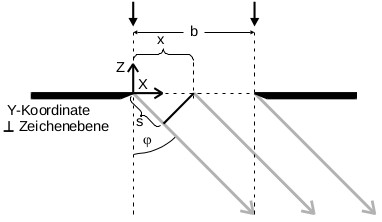
\includegraphics[width=0.7\textwidth]{images/spalt.jpg}
    \label{fig:1}
    \caption{Beispielhafte Darstellung der Beugung an einem Einzelspalt \cite{V406}.
    Auf der Abbildung ist ein Einzelspalt der Breite b dargestellt, durch welchen 
    Licht mit Wellenlänge S unter einem Winkel $\varphi$ gebeugt wird. Das x stellt dabei
    den Abstand zweier Lichstrahlen bei einer gleichmäßigen Betrachtung des Spaltes als Beispiel dar.
    }
\end{figure}
\flushleft{Um\,}\justifying Beugungsphänomene zu beobachten wird eine  Breite b des Spaltes gewählt, welche  im Vergleich zu
seiner Länge groß ist, sodass das ganze auf ein eindimensionales Problem reduziert werden kann.
Als Lichtquelle eignet sich dafür ein Laser. Die vom Laser ausgesendeten ebenen Wellen
treffen auf den Einzelspalt und nach dem Hyugenschen Prinzip bildet jeder Punkt einer Welle
eine Kugelwelle. Das Beugungsmuster der Welle entsteht dann durch die Interferenz der einzelnen
Kugelwellen. Die Beugungsfunktion sieht dabei folgendermaßen aus
\begin{align}
    B(\varphi) &= A_0 b \frac{\sin (\eta)}{\eta}  \label{eq:1} \quad \text{mit}\\
    \eta &= \frac{\pi b \sin \varphi}{\lambda} \label{eq:2} \text{\cite{V406}} .
\end{align}
$\lambda$ ist hierbei die Wellenlänge des einfallenden Lichts und $A_0$ die Amplitude
der einfallenden Welle.

\flushleft{Als\,}\justifying Graph sieht die Funktion dabei wie folgt aus:
\begin{figure}[H]
    \centering
    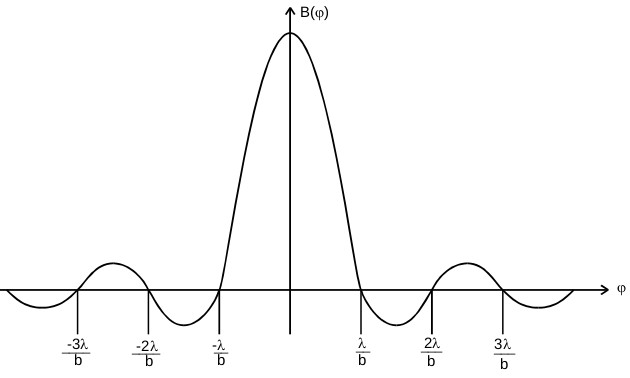
\includegraphics[width=0.7\textwidth]{images/graph.jpg}
    \label{fig:2}
    \caption{Darstellung der Beugungsfunktion\cite{V406}.
    In der Abbildung wird der theoretische Verlauf der Gleichung \eqref{eq:1} gezeigt. 
    Dabei ist $B(\varphi)$ auf der y-Achse und $\varphi$ auf der x-Achse eingetragen.
    Die auf der x-Achse angegebenen Punkte stellen die Nullstellen der Beugungsfunktion dar.
    }
\end{figure}
\flushleft{Die\,}\justifying Nullstellen sind dabei an den Stellen
\begin{align}
    \sin \varphi _n = \pm n \frac{\lambda}{b} \text{\cite{V406}} \label{eq:3},
\end{align}
wobei n eine natürliche Zahl ist.
Da die Beugung $B(\varphi)$ aufgrund der hohen Lichtfrequenzen nur schwer messbar ist,
wird stattdessen die Intensität $I(\varphi)$ 
\begin{align}
    I(\varphi)  B(\varphi) = A_0^2 b^2 \left\{\frac{\lambda}{\pi b \sin \varphi} \right\} \sin ^2 \left(\frac{\pi b \sin \varphi}{\lambda} \right) \text{\cite{V406}} \label{eq:4}
\end{align}
gemessen.\\


\section{Versuchsaufbau und Durchführung}
Bei dem Einzelspalt-Experiment wird ein Laser auf einem Stativ befestigt und dieses auf 
eine Messschiene befestigt. Dann wird eine Bledenhalterung mit einem Stativ 
mit etwas Abstand zum Laser auf der Schiene befestigt. Zuletzt wird in einer Entfernung L auf der Messchiene
ein Photoelement auf einem Verschiebereiter befestigt. Dieser wird an ein Amperemeter
angschlossen. Dies sieht beispielsweise so aus:
\begin{figure}[H]
    \centering
    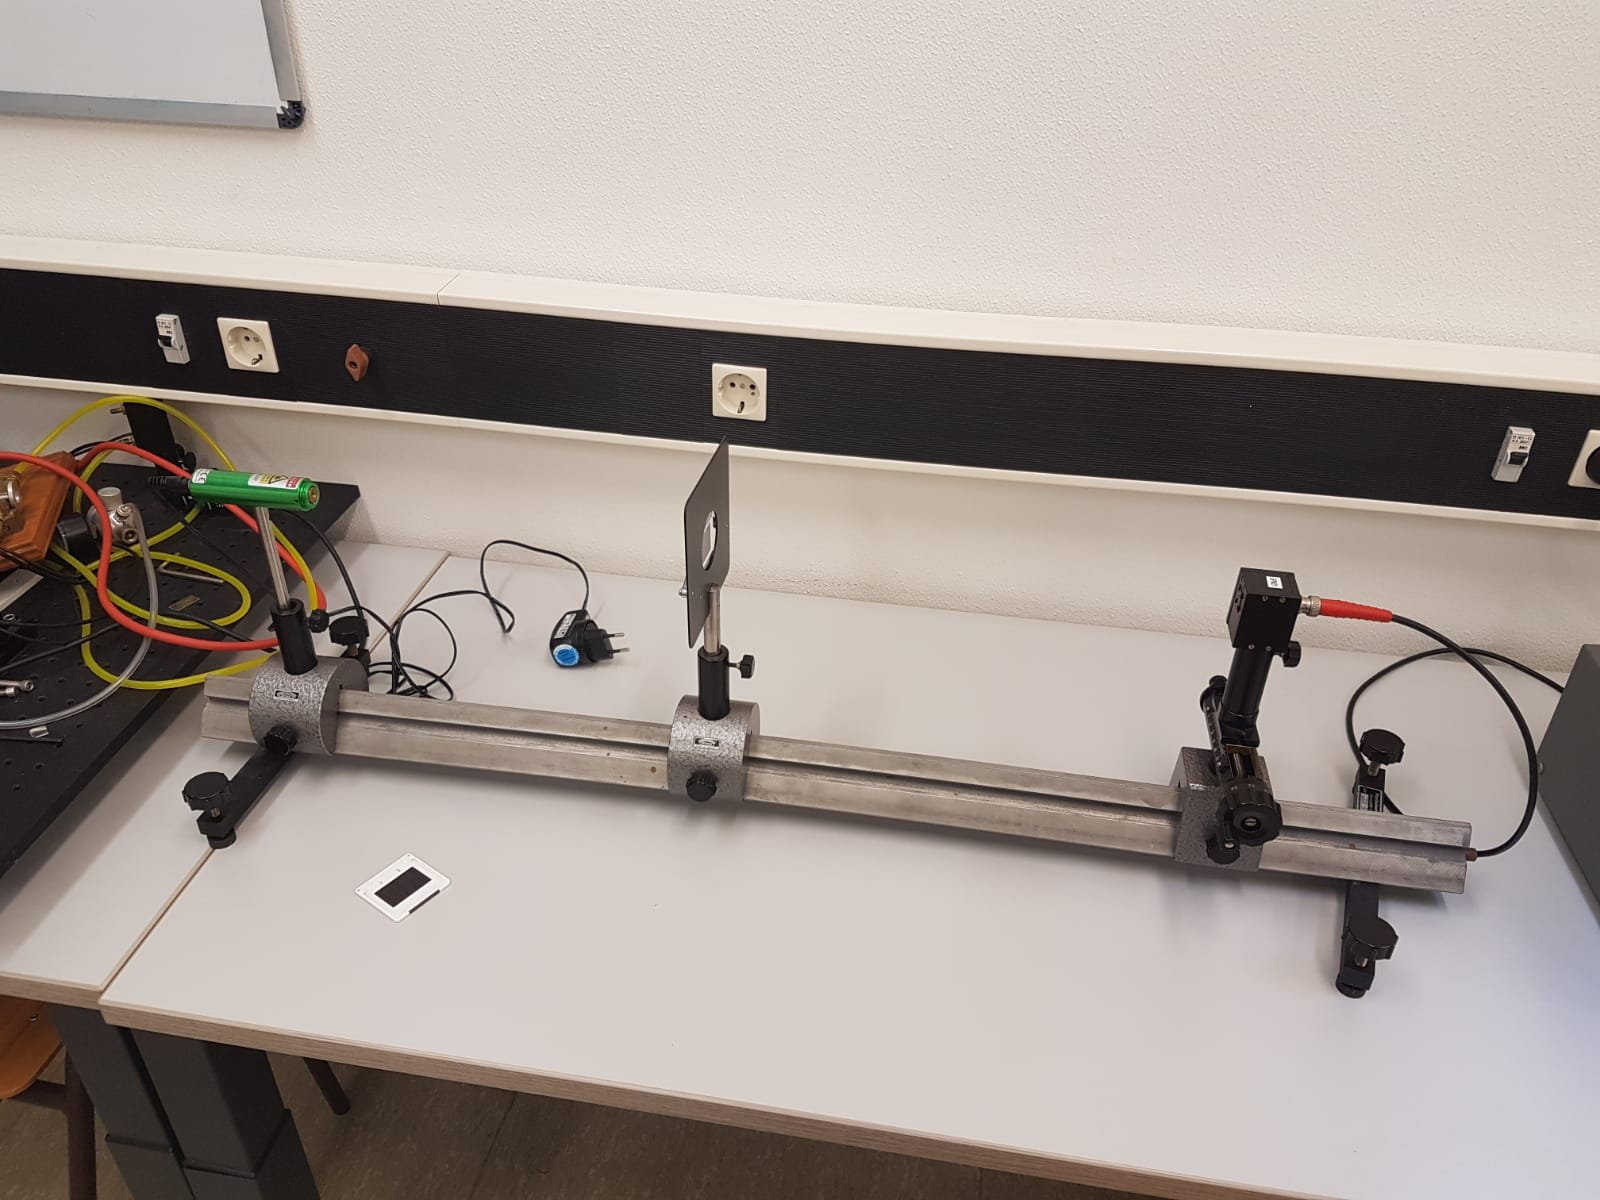
\includegraphics[width=0.7\textwidth]{images/aufbau.jpg}
    \caption{Beispielhafter Aufbau eines Einzelspalt-Experiments.\\
    Links ist ein Laser auf einem Stativ, welches sich auf einer Messschiene befindet, angebracht.
    In der Mitte befindet sich die Blendenhalterung und rechts das Photoelement auf einem 
    Verschiebereiter. Das Licht des Lasers erzeugt dann durch die Blende in der Halterung 
    ein Interferenzbild, welches vom Photoelement an den verschiedenen Winkeln gemessen wird
    }
    \label{fig:3}
\end{figure}
\flushleft{Zuerst\,}\justifying wird der Laser in Richtung der Blende und parallel zur Messschiene
ausgerichtet. Dann wird der Punkt, auf dem der Laser auf dem Verschiebereiter zeigt, mit dem
Photoelement bestimmt. Dann wird ein Einzelspalt in die Halterung eingebracht, so dass
das Licht durch den Spalt geht. Danach werden ausgehend vom Hauptmaximum rechts und links 
ca. 50 Messwerte aufgenommen.

\section{Auswertung}
Alle Plots in der Auswertung werden mit matplotlib \cite{matplotlib} erstellt und alle
Fehler mit uncertainties \cite{uncertainties} berechnet.\\
Bei der Durchführung des Einzelspalts wird ein Laser der Wellenlänge $\lambda = \SI{532}{\nano\meter} $ verwendet.
Der Einzelspalt hat eine Breite von $d=\SI{0.1}{\milli\meter} $ und der Abstand von 
der Blende zum Verschiebereiter beträgt $L=\SI{39.3+-0.1}{\centi\meter} $.\\
Die Tabelle \ref{tab:1} mit den Messwerten für die folgende Graphik befindet sich im Anhang.
\begin{figure}[H]
    \centering
    \includegraphics[width=\textwidth]{plot.pdf}
    \caption{
        Plot der Intensität des Beugunsbildes eines Einzelspalts der Breite \SI{0.1}{\milli\meter}.\cite{matplotlib}\\
        Aufgetragen ist hier die Intensität in Form der gemessenen Stromstärke
        gegen den Beugungswinkel \varphi in rad. Der Beugungswinkel wird hierbei mithilfe von
        Formel \eqref{eq:5} berechnet. Die Fitkurve wird mithlife von curvefit aus Scipy \cite{scipy}
        und der Gleichung \eqref{eq:6a} erstellt. 
    } 
    \label{fig:4} 
\end{figure}
\flushleft{Für\,}\justifying die x-Werte werden die kleinen Winkel $\varphi$ durch 
\begin{align}
    \varphi \approx \tan (\varphi) = \frac{b-b_0}{L} \label{eq:5}
\end{align}
genähert. Hierbei sind $b$ die Werte auf dem Verschiebereiter und $b_0$ der Punkt des Maximums.
Hier wird das Maximum bei $b_0= \SI{27.7}{\milli\meter} $ gewählt.\\
Die Fitkurve wird hier mit der Funktion curvefit aus Scipy \cite{scipy} erstellt.\\
Die Fitfunktion und die Fitparameter lauten hierbei:
\begin{subequations}
\begin{align}
    I(\varphi) &= A^2 \,\text{sinc} \left(\frac{b \sin{\varphi}}{\SI{532}{\nano\meter}} \right) \label{eq:6a}\\
    A &= 8,31 \pm 31390,38 \label{eq:6b}\\
    b &= \SI{0.13+-1096.6}{\milli\meter} \label{eq:6c}
\end{align}
\end{subequations}
Hierbei ist die Funktion Sinus cardinalis definiert als
\begin{align}
    \text{sinc}\,x = \frac{\sin (\pi x)}{\pi x} \label{eq:7} .
\end{align}
Dabei entsteht aus der Fitfunktion die Formel \eqref{eq:4}, wenn für
\begin{align}
    A &= b^2 A_0^2 \label{eq:8} \\
    x &= \frac{b \sin{\varphi}}{\SI{532}{\nano\meter}} \label{eq:9}
\end{align}
wählt wird.
Der Punkt, bei dem im Fit durch 0 geteilt wird, wird dabei automatisch ignoriert.



\section{Diskussion}
Der angegebene Wert für die Breite des Einzelspalts beträgt
\begin{align}
    b_{\text{lit}} = \SI{0.1}{\milli\meter}. \label{eq:10}
\end{align}
Daraus lässt sich der relative Fehler mit dem berechneten $b$ aus Gleichung \eqref{eq:6c} berechnen
\begin{align}
    b_{\text{rel. Fehler}} &= \frac{b-b_{\text{lit}}}{\text{lit}} \label{eq:11}\\
    b_{\text{rel. Fehler}} &= \text{\input{relerr_b.tex}}.
\end{align}
Dieser Fehler ist grundsätzlich groß. Eine Erklärung für diesen könnte unter anderem
die Näherung in Gleichung \eqref{eq:5} darstellen, da es eben nur eine Näherung
ist und nicht die genauen Verhältnisse wiederspiegelt. Zudem sind alle Messungen
unter Lichteinfall durchgeführt worden, welche auch von dem Photoelement als Untergrund
gemessen worden ist. Zudem könnte der Laser nicht perfekt auf den Spalt ausgerichtet worden
sein, wodurch das Beugungsbild verändert werden würde.\\ Sehr auffälig sind die immens 
großen Messungenauigkeiten bei den Parametern \eqref{eq:6b} und \eqref{eq:6c} der Fitkurve,
welche mehrere Größenordnungen über den eigentlichen Wert liegen. Diese können nicht durch statistische
Fehler entstanden sein, da dafür der Fit zu gut auf die Werte passt. Auch systematische Fehler
können dies nicht erklären, da dafür die Werte zu nah am Literaturwert liegen. Daher ließe sich vermuten, dass
es an der Funktion curvefit liegt bzw. ihrer verwendeten Funktion.

\newpage
\printbibliography

\newpage
\section*{Appendix}
\addcontentsline{toc}{section}{Appendix}
\input{table.tex}

\end{document}


